\section{Presentation Logic Layer}

%What pages will be present in your project? briefly indicate how your web site will be organized

The web application is divided in the following pages:
\begin{itemize}
	
	
	
	
	\item Homepage: 
	\item The gym :
	\item Courses :
	\item Calendar :
	\item Prices : This page shows the prices of each type of subscription for each course.
	\item Staff :
	\item Contact Us :
	\item Login :
	\item Register :
	\item Trainee :
	\item Trainer :
	\item Secretary :
	---------------- DA RISCRIVERE QUESTE SOTTO CON LE PAGINE SOPRA--------------
	\item Homepage:contains the main information reguarding the gym such as the available courses held in a given period, instructors, rooms, timetables, pricing...
	\item Login: portal where a guest user can login, with his own credentials, and enter in the personal area (different for all roles).
	\begin{itemize}
		\item Reset password: minimal page where a user can change his own password, forgotten.
	\end{itemize}
	\item Sign in: page where an unregistered user can sign in, access to the trainee area and enjoying all the functionalities.
	\item Trainee area/subscriptions: user can buy subscriptions to different courses
	\item Trainee area/bookingSlot: after having bought a subscription, user can book time slots (of the subscripted course) with his own preference.
	\item Secretary page: a secretary mark the presence of the people arrived in the gym to attend a particular time slot
	
	\item VARIOUS PAGES!
\end{itemize}

\newpage
\subsection{Mockups}
\subsubsection{Home Page}
\subsubsection{The Gym}
\subsubsection{Calendar}
\subsubsection{Prices}
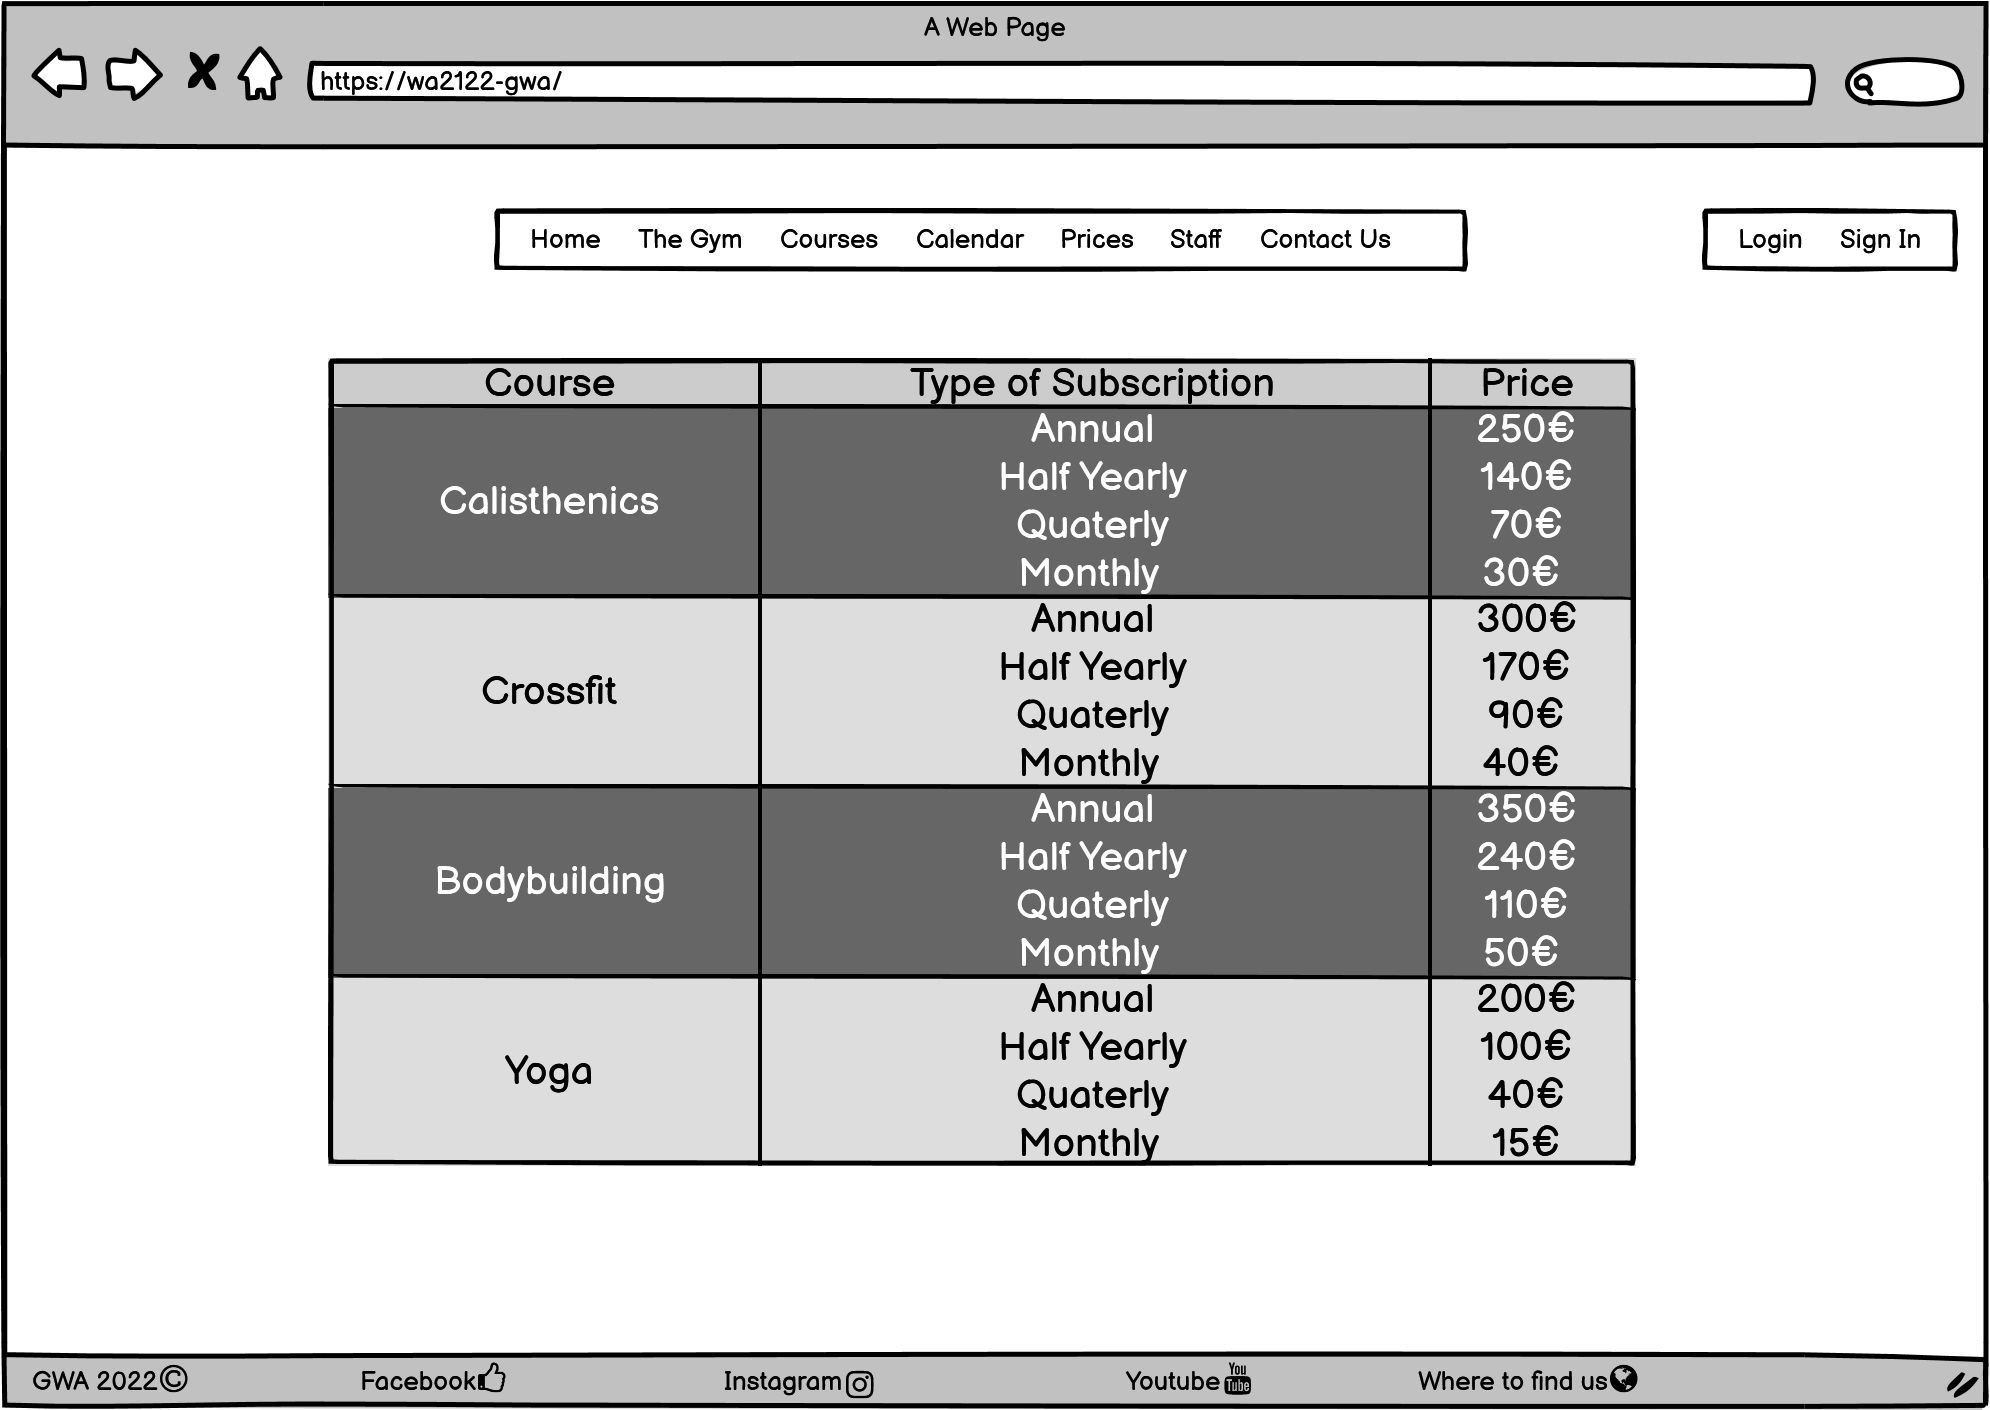
\includegraphics[width=\columnwidth]{InterfaceMockup/Prices/prices_page.png}
\subsubsection{Staff}
\subsubsection{Contact Us}
\subsubsection{Login}
\subsubsection{Register}
\subsubsection{Trainee}
\subsubsection{Trainer}
\subsubsection{Secretary}







